\documentclass{article} % For LaTeX2e
\usepackage{nips15submit_e,times}
\usepackage{hyperref}
\usepackage{url}
\usepackage{graphicx}
%\documentstyle[nips14submit_09,times,art10]{article} % For LaTeX 2.09
\usepackage{color}
\usepackage{amssymb,amsmath,graphicx}
\usepackage{amsfonts}
\usepackage{url}



\newcommand{\fref}[1]{Fig.~\ref{fig:#1}}
\newcommand{\flabel}[1]{\label{fig:#1}}

\newcommand{\figdir}{}
\newcommand{\capt}[2]{\caption[#1]{\textbf{#1}#2}}
\newcommand{\qcapt}[1]{\capt{#1}{}}
\newcommand{\figheadingnospace}[1]{\center{\textbf{#1}}}
\newcommand{\figheading}[1]{\figheadingnospace{#1}\vspace{3mm}}
\newcommand{\fig}[5]
{
\begin{figure}
\begin{center}
\includegraphics[width=#3\columnwidth]{\figdir#1}
\end{center}
\capt{#4}{#5}
\flabel{#2}
\end{figure}
}


\title{Handwriting Generation with Recurrent Neural Networks}


\author{
Jing Leng \\
University of Michigan\\
\texttt{lengjing@umich.edu} \\
\And
Shayan Masooman \\
University of Michigan \\
\texttt{masooman@umich.edu} \\
\And
Blake Smith\\
University of Michigan \\
\texttt{blakesm@umich.edu} \\
}

% The \author macro works with any number of authors. There are two commands
% used to separate the names and addresses of multiple authors: \And and \AND.
%
% Using \And between authors leaves it to \LaTeX{} to determine where to break
% the lines. Using \AND forces a linebreak at that point. So, if \LaTeX{}
% puts 3 of 4 authors names on the first line, and the last on the second
% line, try using \AND instead of \And before the third author name.

\newcommand{\fix}{\marginpar{FIX}}
\newcommand{\new}{\marginpar{NEW}}

\nipsfinalcopy % Uncomment for camera-ready version

\begin{document}

\maketitle

\begin{abstract}
In this report we talk about using recurrent neural networks to generate a font that resembles human handwriting. There have been various methods proposed to make machines mimick handwriting in previous research however we chose to approach this problem through the use of Long Short-term Memory recurrent neural networks to make predictions dealing with sequential data. To collect data, we employed video processing software and then used handwriting recognition algorithms on an image of the handwriting to link it with its print-text equivalent. As you will see, the experiments we completed produced satisfactory results in the sense that our algorithm produces an eligible handwriting font for a given input. 

\end{abstract}

 % * Sec 1. Introduction: introduce the problem you want to solve, expain why it is important to solve it; and indicate the method 
 %    you used to solve it. add a concept figure showing the overall idea behind the method you are presenting. 
 %  * Sec 2.1. Review of previous work (i.e. previous methods that have explored a similar problem)
 %  * Sec 2.2. Say why your method is better than previous work; and/or summarize the key main contributions of your work; 
 %  * Sec 3.1: Technical part: Summary of the technical solution 
 %  * Sec 3.2: Technical part: Details of the technical solution; you may want to decompose this section into several subsections; 
 %    add figures to help your explanation. 
 %  * Sec 4: Experiments: present here experimental results of the method you have implemented with plots, graphs, images 
 %    and visualizations.
 %  * Sec 5: Conclusions: what's the take home message? 
 %  * Sec 6: References

\section{Introduction}

Optical character recognition (OCR) is a widely used form of human-computer interaction that can be seen in society today. It is the conversion of images of typed or printed text into machine-encoded text often used for data entry, text-to-speech, and text mining. In this project we have implemented Intelligent Character Recognition (ICR) software that has the capability to take OCR to the next level and recognize handwritten text one character at a time. This is all done with the intention of using handwriting recognition to construct an exclusive and accurate handwriting font tailored to unique input in order to grant out users the ability to add a personal touch to the banal style of standard electronic fonts.

This complex input will be seamlessly fed to our software through the utilization of the “Wacom Intuos Draw Tablet  Stylus” here on the University of Michigan campus. The “Wacom Intous Draw Tablet” grants¬ the capability to track dynamic motion of the pen tip in real-time as our users input their handwriting, which will be used to construct a data set and recreate the handwriting to a digital image. It is at this point that the handwriting recognition software can be used to analyze the handwriting and generate a text file of matching text ultimately feeding these two correlated inputs to the rest of our software to begin creating a realistic font simply off a sample of our user’s handwriting. 

Creation of a realistic font is most efficiently done through the process of machine learning in which the computer trains a model from extensive previous input to make data-driven decisions (i.e. predictions) rather than following strictly static program instructions. With the ability to process and store handwritten text by comparison between scanned text and learned text, our software will ultimately construct a font that is particular to the handwriting input to be used for future use on the system. A requisite for a font to resemble actual handwriting is that each letter must be displayed diversely each time it is used, and it’s size and shape will depend on the values of surrounding letters. Conclusively, this project has provided us with useful experience in the practice of video processing, handwriting recognition, and machine learning using video as input to create a unique tool to use in a vast variety of circumstances. A concept figure illustrating the method described is shown below.

	%insert picture of method
\begin{center}
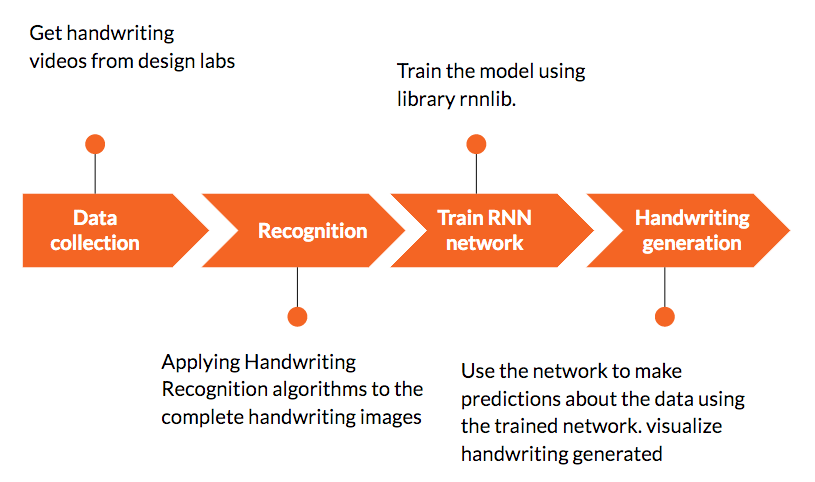
\includegraphics[scale = 0.5]{Method.png}
\end{center}



% introduce the problem you want to solve, expain why it is important to solve it; and indicate the method you used to solve it. add a concept figure showing the overall idea behind the method you are presenting. 
\section{Previous work}
\subsection{Handwriting recognition} % Review of previous work (i.e. previous methods that have explored a similar problem)
Recognizing handwriting from an image poses several problems and is no simple task. The most important obstacle is that there is a significant amount of variation within classes, as you can see below, there are several different ways the letters "A" and "Z" can be handwritten.
\begin{center}
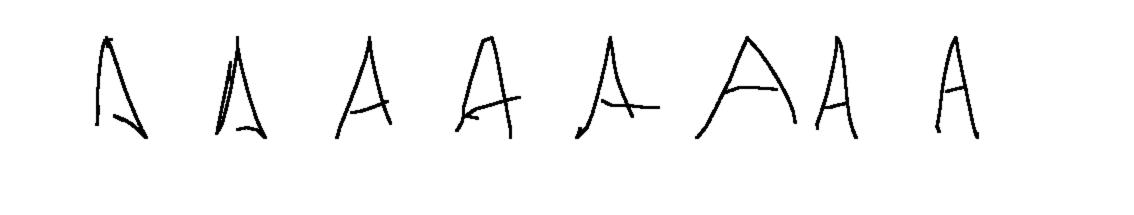
\includegraphics[scale = 0.25]{A.jpg}
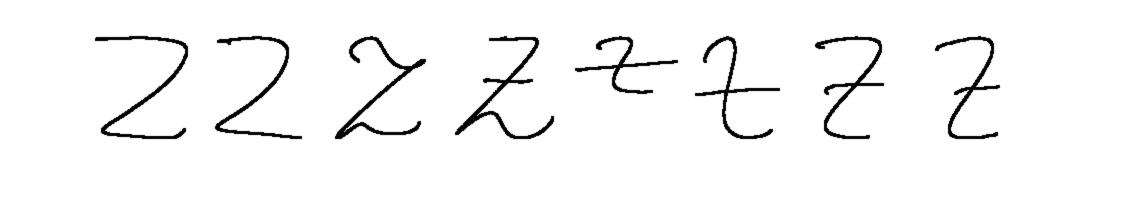
\includegraphics[scale = 0.25]{Z.jpg}
\end{center}
The MATLAB OCR function in the Computer Vision toolbox works extremely well with recognizing typed text in an image, as shown below.
\begin{center}
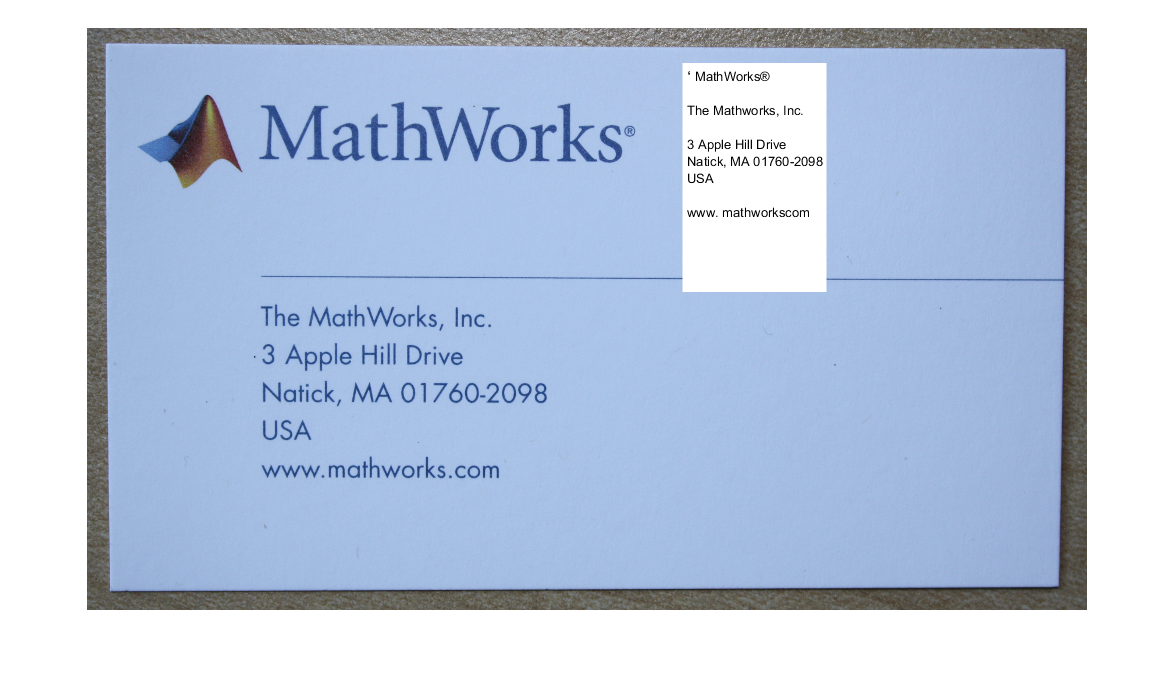
\includegraphics[scale = 0.4]{RecognizeTextWithinAnImageExample_01.png}
\end{center}
However, the OCR function works very poorly with actual handwriting recognition, making it unsuitable for this project. The method we implemented is similar to the paper "Optical Character Recognition for Handwritten Hindi". This paper recognizes hindi text by using Histogram of Oriented Gradient (HOG) Features with three different classifiers: Naive Bayes, Support Vector Machines, and Adaboost. The Support Vector Machines gave the highest test accuracy (1.2 percent misclassification rate), so we decided to use the SVM classifier for our method.
\subsection{Handwriting generation} % Say why your method is better than previous work; and/or summarize the key main contributions of your work;
There have been plenty of ways to approach the problem of handwriting synthesis. They can be categorized into Perturbation-based techniques, Fusion-based generation, and Model-based generation. 
Perturbation-based techniques generate new samples by
altering geometric features such as the size, thickness, and
slant of a given sample. Perturbation-based operations can
be seen as the inverse of the preprocessing steps employed
in text recognition. Perturbation-based techniques are easy
to apply, but the results may be unnatural due to random and
non-calibrated parameter settings. 

Fusion-based techniques take few input samples and combine
them into new synthesized outputs. They differ from concatenation
techniques in that they generate scripting units at the
same level as their inputs; e.g., characters generate new characters.
Shape-matching algorithms are necessary for fusionbased
techniques to make sure that segments are properly
aligned. The number of unique outputs is limited in fusionbased
techniques as compared to that of other generation
techniques.

Model-based techniques capture the statistics of natural
handwriting variations into models. Although model-based
techniques are profoundly established in theory, they may
often be challenging to implement due to the large number
of samples they require. Models resulting from
these techniques can also be utilized in recognition systems. 


\section{Technical details}
\subsection{Data Collection}

The first step to our software process is for our user to input their handwriting. We need to process this input in real time in order to gather sufficient data of where the pen tip is at all times while it is writing and an indication of when it is picked up. This will ensure that with the help of our trained machine, the font we generate is realistic in the sense of all inconsistencies that normal handwriting possesses. Therefore we set out to obtain ∆x and ∆y of the pen-tip corresponding to its timestamp and when the pen is lifted so that the next ∆x and ∆y pair that you will see will be the initial point of a new stroke. 

To capture the user’s handwriting we chose to utilize the accessible and accurate “Wacom Intuos Draw Tablet and Stylus” available on North Campus, with Adobe Photoshop. After opening a blank canvas and selecting the pen tool, the individual uses the stylus to write out a phrase and with Apple QuickTime Player’s built in screen capture we obtain a video of the handwriting phrase frame by frame as it is written. The input to be used by the initial stage of our software has thus been obtained. 

As mentioned, this video needs to be processed and converted to a formatted data file. To accomplish this we utilized the video processing capabilities of Matlab’s videoReader functionality. Employing frame by frame comparisons to detect pixel discrepancies, a competently accurate representation of the handwriting is exported to an excel document in all necessary variables. With this data in its appropriate format, the last frame of the video is used as image input to another portion of our software to recognize the handwriting and construct a text file to pair with the output of data collection.

\subsection{Handwriting recognition}

In order to use the Histogram of Oriented Gradients (HOG) Features and Support Vector Machine Classifier (SVM), we needed a large dataset which contained images of handwritten letters. The UCI Machine Learning Repository had sample penstroke data from 60 different writers, each ASCII character as well as a few spanish characters were included in the dataset. We only used the uppercase and lowercase letters of the English alphabet, and converted the penstroke data into $120\times 120$ pixel images for each letter. This gave us a training set of 60 $120\times 120$ pixel images for each letter.

On each of the images of the training set, we found the HOG features using a window size of 20, and input these into an SVM in order to get a classifier. The visualization of the HOG features is shown in the image below. The window size of 20 gave adequate information on the shape of each letter while still providing a reasonable runtime. 
\begin{center}
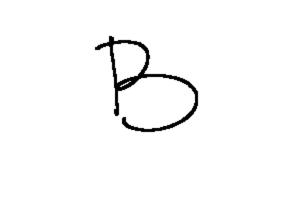
\includegraphics[scale = 0.25]{B1.jpg}
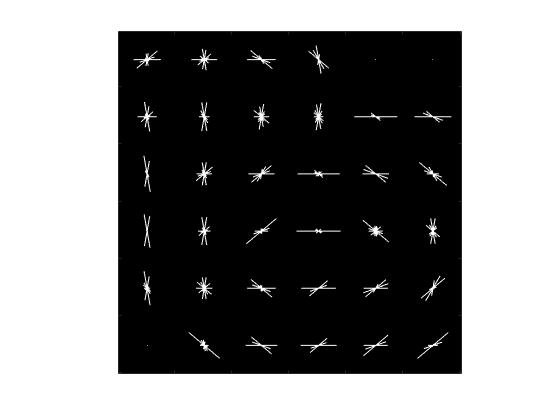
\includegraphics[scale = 0.25]{B1hog.jpg}
\end{center}
On any new image, the MATLAB function \textbf{improps} was used to separate letters, then our classification was used on each separate letter.
\begin{center}
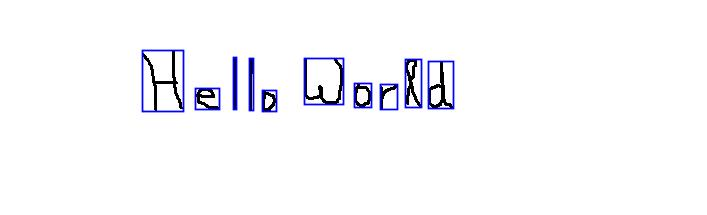
\includegraphics[scale = 0.5]{boxexample2.jpg}
\end{center}
\subsection{Handwriting generation}

Neural networks (NN) are know to do a good job in capturing complex, non-linear connections between input and output. A recurrent neural network (RNN) is a class of artificial neural network where connections between units form a directed cycle. This creates an internal state of the network which allows it to exhibit dynamic temporal behavior. Unlike feedforward neural networks, RNNs can use their internal memory to process arbitrary sequences of inputs. This makes them applicable to tasks such as unsegmented connected handwriting recognition or speech recognition. 

\begin{figure}[h]
\begin{center}
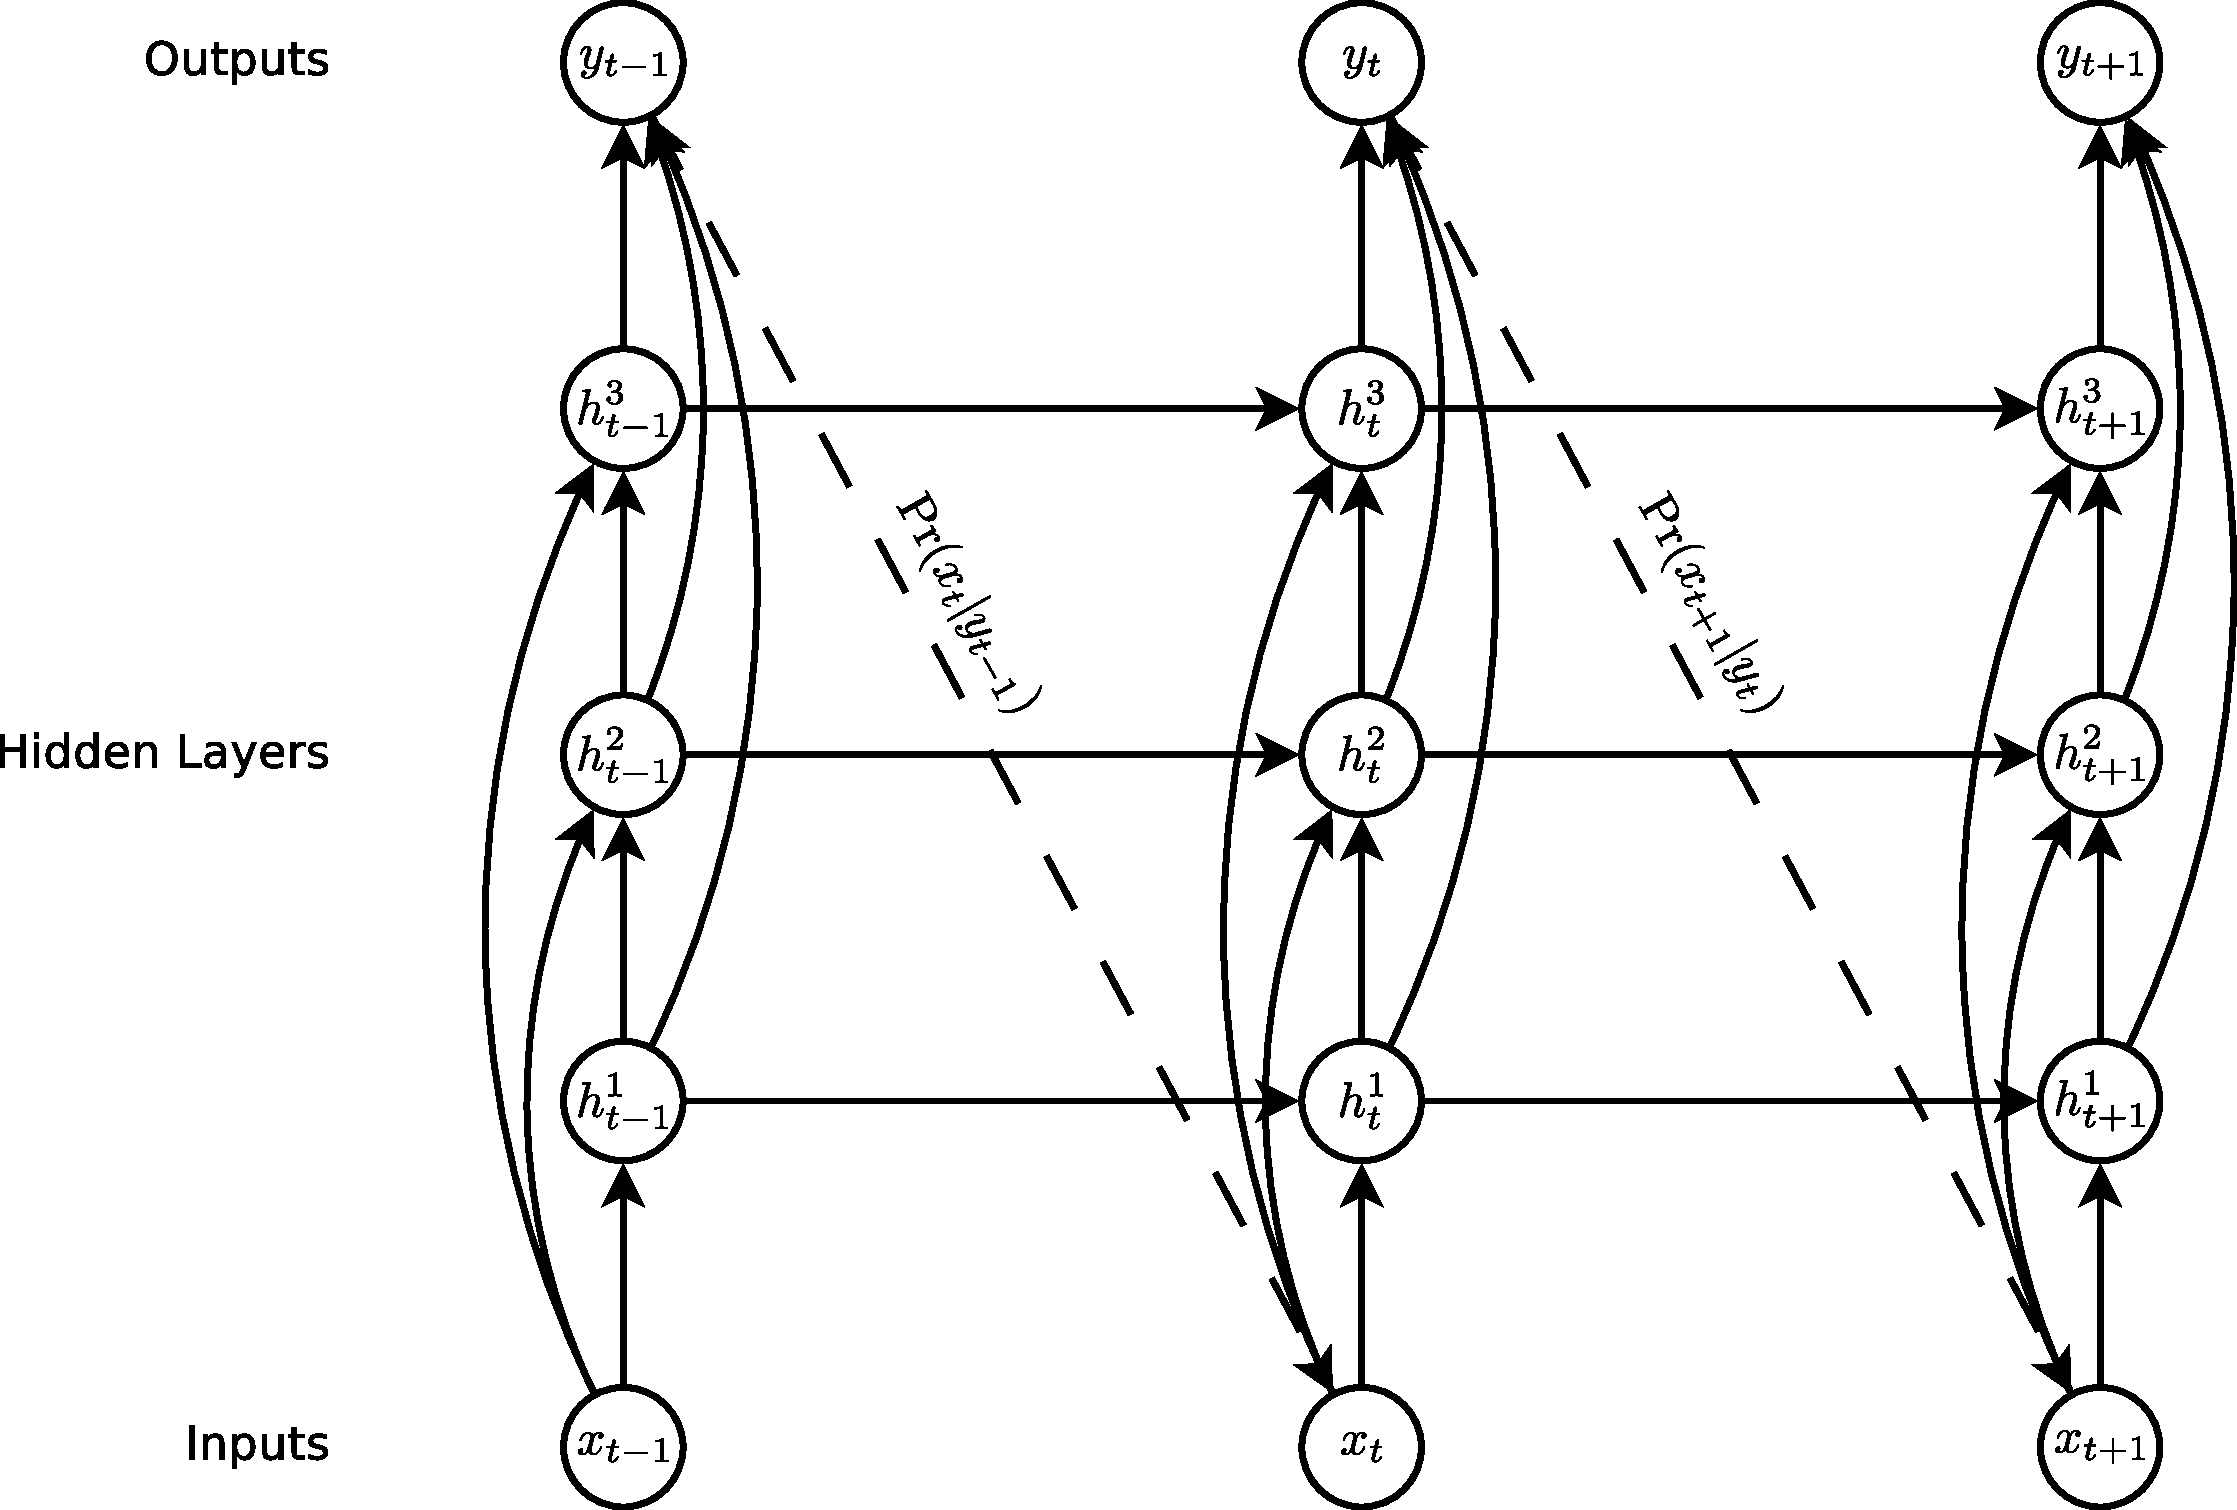
\includegraphics[scale = 0.3]{deep_predictor.pdf}
\caption{\textbf{Deep recurrent neural network prediction architecture.} The circles represent network layers, the solid lines represent weighted connections
and the dashed lines represent predictions. }
\flabel{deep_predictor}
\end{center}
\end{figure}

In \fref{deep_predictor}, an input vector sequence $\mathbf{x}=(x_1, \ldots, x_T)$ is passed long a weighted connections to a stack of $N$ recurrently interconnected hidden layers to compute the first hidden vector sequences $\mathbf{h}^n = (h^n_1,\ldots,h^n_T)$, and then the output vector sequence $\mathbf{y} = (y_1, \ldots, y_T)$

Each output vector $y_t$ is used to parameterise a predictive distribution $\Pr(x_{t+1}|y_t)$ over the possible next inputs $x_{t+1}$.

The first element $x_1$ of every input sequence is always a null vector whose entries are all zero; the network therefore emits a prediction for $x_2$, the first real input, with no prior information.
The network is `deep' in both space and time, in the sense that every piece of information passing either vertically or horizontally through the computation graph will be acted on by multiple successive weight matrices and nonlinearities.

How each hidden node is calculated can be shown in the following formula: 
\begin{align}
\label{eq:pred_hidden}
h^1_t &= \mathcal{H}\left(W_{i h^1} x_t + W_{h^{1}h^{1}} h^1_{t-1} + b_{h}^1 \right)\\
h^n_t &= \mathcal{H}\left(W_{i h^n} x_t + W_{h^{n-1}h^{n}} h^{n-1}_t + W_{h^{n}h^{n}} h^n_{t-1} + b_h^n \right)
\end{align} 
where the $W$ terms denote weight matrices (e.g.\ $W_{i h^n}$ is the weight matrix connecting the inputs to the $n^{th}$ hidden layer, $W_{h^{1}h^{1}}$ is the recurrent connection at the first hidden layer, and so on), the $b$ terms denote bias vectors (e.g.\ $b_o$ is output bias vector) and $\mathcal{H}$ is the hidden layer function. 

Given the hidden sequences, the output sequence can be calculated: 
\begin{align}
\label{eq:pred_output}
\hat{y}_t &= b_o + \sum_{n=1}^N{W_{h^n y} h^n_t}\\
y_t &= \mathcal{Y}(\hat{y}_t)	
\end{align}

The Long short-term memory (LSTM) network, developed by Hochreiter \& Schmidhuber in 1997, is an artificial neural net structure that unlike traditional RNNs doesn't have the vanishing gradient problem (compare the section on training algorithms below). It works even when there are long delays, and it can handle signals that have a mix of low and high frequency components. LSTM RNN outperformed other methods in numerous applications such as language learning and connected handwriting recognition.


That is how the network is built. 

In this project, the data is the sequence 

To enable the network to make prediction about a sequence, the output sequence is used as a parameter of the probability distribution $\Pr(x_{t+1}|y_t)$ of the next input. The form of distribution should be selected carefully to give high performing prediction. 

The probability given by the network to the input sequence x is
\begin{equation}
\Pr(\mathbf{x}) = \prod_{t=1}^T{\Pr(x_{t+1}|y_t)}
\end{equation}



\section{Experiments}
\subsection{Data collection}

As discussed in Section 3.1, the input to be translated to collected data is in video format and is processed by detecting pixel discrepancies between each frame. An example of detected pixel discrepancies is shown below where detected discrepancies between a frame range was highlighted to show accuracy in the construction of the letter ‘H.’ Note that the cursor does not interfere with detection due to disregard of pixels that have been accurately identified as pixels changed due to cursor for every iteration/frame.
%insert picture of 'detection data'
\begin{center}
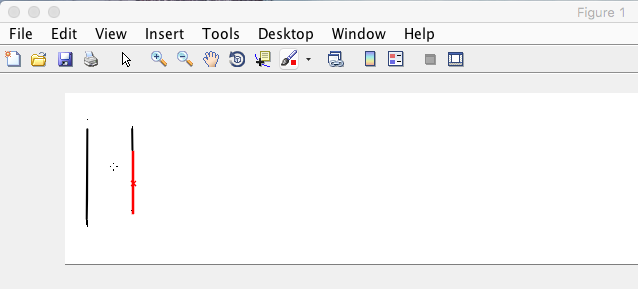
\includegraphics[scale = 0.4]{detection_data.png}
\end{center}

At the completion of the video processing there should be two accessible outputs for use later in software. The first is the last frame of the handwriting input and the second is the formatted data. Examples of these are shown below. 
%insert picture of 'Hello World'
\begin{center}
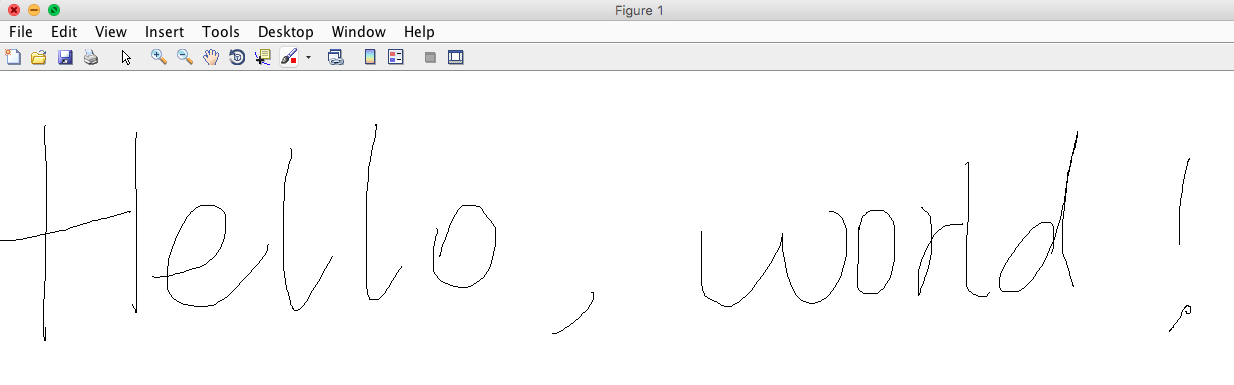
\includegraphics[scale = 0.2]{Hello_world.png}
\end{center}
%insert picture of 'Collected Data'
\begin{center}
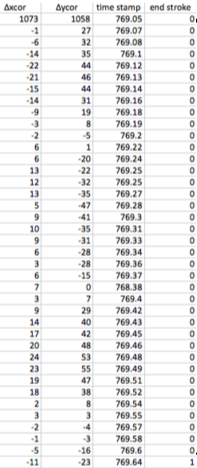
\includegraphics[scale = 0.7]{Collected_Data.png}
\end{center}


\subsection{Handwriting recognition}
As discussed in Section 3.2, letters were separated using the \textbf{improps} MATLAB function, and our SVM classifier was used on each separate letter. The results were extremely accurate on typed text, as shown below (green=correct classification was made, red=incorrect classification was made).
\begin{center}
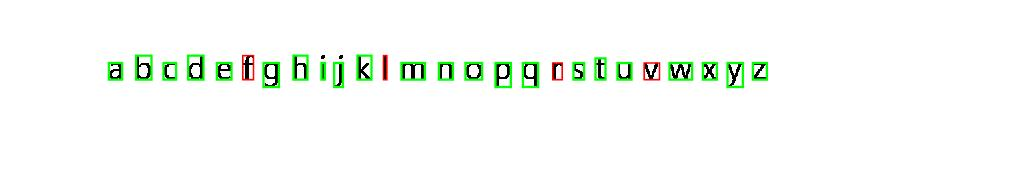
\includegraphics[scale = 0.5]{alowerignore.jpg}
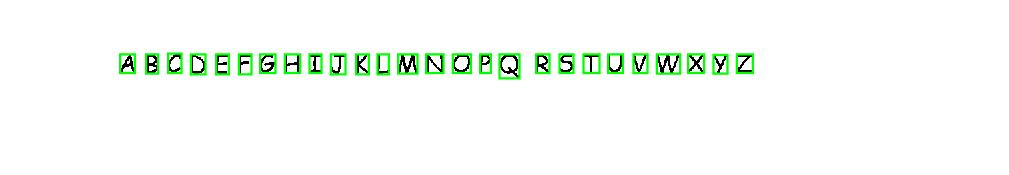
\includegraphics[scale = 0.5]{aupperignore.jpg}
\end{center}
However, there was still a very high misclassification rate on handwritten text (30 percent). As you can see below, several letters are still being misclassified. While this is a fairly good handwriting recognizer, it still causes a huge problem in our project, since some of the letters from the "Hello World" example from Section 3.1 will be misclassified, the error will propogate to the handwriting generator, as dicussed in the following section.
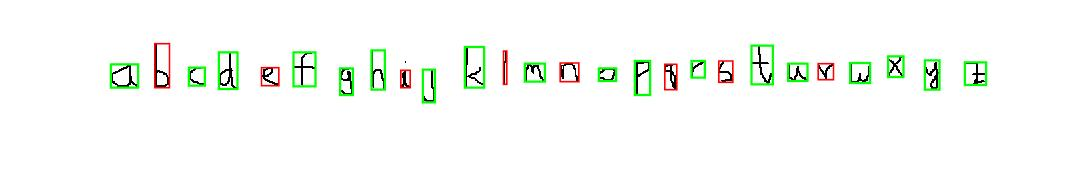
\includegraphics[scale = 0.5]{alowerwrittenignore.jpg}
\begin{center}

\includegraphics[scale = 0.5]{HelloWorldwrittenbox.jpg}
\end{center}
\subsection{Handwriting generation}
First we collected a trace of the pen stroke using a tracking pad and screen capture. Then we used the handwriting recognition technology to generate the contents of handwriting. With the data collected we trained a Recurrent Neural Network, which is later used for handwriting generation. 

After we collected and formatted the data, we use the data to train a recurrent neural network. The idea of RNN is to encode sequential correlation of ordered data points, in our case, the pen stroke data introduced earlier. The input and output variable will be the same sequence, except they are offsetted by one timestamp to make prediction possible. By training the recurrent neural network we are basically telling the program how to write. 

Using the well-implemented C++ library rnnlib, we were able to train an RNN that takes in the sequential data of the pen stroke, which is then used for making predictions about handwriting, i.e. handwriting generation. The training of the network took longer than we thought. Each epoch takes 30 hours or so, and therefore we only managed to run 7 epochs. The training error was still dropping when we stop the training process early because of time issues, so the network is not yet well trained. Nevertheless it has given us eligible results. 


Here are two examples: 
\begin{figure}[h]
\begin{center}
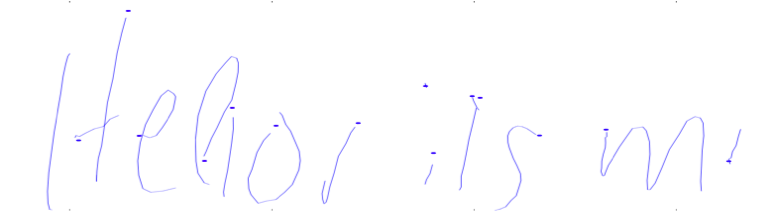
\includegraphics[scale = 0.5]{hello.png}
\end{center}
\flabel{hello}
\caption{"hello, it's me"}
\end{figure}

\begin{figure}[h]
\begin{center}
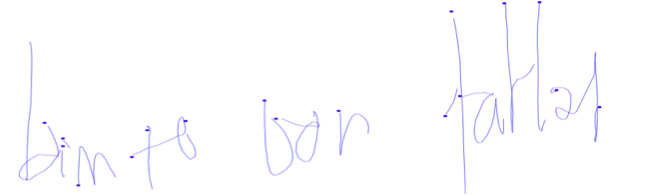
\includegraphics[scale = 0.5]{father.png}
\end{center}
\flabel{father}
\caption{"I am your father"}
\end{figure}

\fref{hello}, which says "hello, it's me", is very legible, and looks like a sensible handwriting version of the text. Looking closely, we can see the ‘e’ at the end was not finished. That is because the end of stroke flag appeared too soon. In another case where the algorithm did not do so well, \fref{father} is less handwriting-like, and less legible.  

\section{Conclusions}
In this project, Long Short-Term Memory recurrent neural networks have displayed a strong ability in making predictions about human handwriting sequence. Although it did not reach its full potential, the RNN we trained is able to generate convincing handwriting data as expressed in our experimental data above. There are a few ways we could improve the project, however. A simple improvement given more time would be to train the network more to improve our output. Additionally, we have come to realize that the rnn library we are using is not optimized for multiprocessors, or gpu, so a strive to improving on their code would go a long way. And finally if we really dove into this project we could also try to improve the architecture of the neural networks, however if that succeeded we would be famous. All in all, this project has given us great insight to video processing, handwriting recognition, and machine learning all contributing to a better understanding of computer vision and the frontier of discovery and improvement that it proposes. 

\subsubsection*{References}

\small{
[1] Graves, A.: Generating Sequences With Recurrent Neural Networks. arXiv preprint arXiv:1308.0850 (2013).

[2] Vincent, N., Seropian, A., Stamon, G.: Synthesis for handwriting
analysis. Pattern Recognit. Lett. 26(3), 267–275 (2005)

[3] Goyal, A., Khandelwal, K., Keshri, P., (2010) "Optical Character Recognition
 for Handwritten Hindi". Stanford, CA.


\end{document}
